\documentclass[12p,a4paper]{article}
\usepackage[utf8]{inputenc}
\usepackage[T1]{fontenc,url}
\usepackage{multicol}
\usepackage{parskip}
\usepackage{lmodern}
\usepackage{microtype}
\usepackage{verbatim}
\usepackage{amsmath, amssymb}
\usepackage{tikz}
\usepackage{physics}
\usepackage{mathtools}
\usepackage{algorithm}
\usepackage{algpseudocode}
\usepackage{listings}
\usepackage{enumerate}
\usepackage{graphicx}
\usepackage{float}
\usepackage{hyperref}
\usepackage{siunitx}
\usepackage[margin=2cm]{geometry}
\renewcommand{\baselinestretch}{1}
\setlength\parindent{0pt}


\begin{document}



\section{Setup}
\subsection{Configuring Github}
To identify yourself, run
\begin{verbatim}
git config --global user.name [github_username]
git config --global user.email [github_email@adress.com]
\end{verbatim}
You can also change the default text editor for opening files. It's vim by default, and it's usually fine to leave it as vim (GitHub rarely opens any document you wish to actually write in, and vim runs in the terminal, which is nice).
\begin{verbatim}
git config --global core.editor [emacs, gedit, atom, whatever you want]
\end{verbatim}


\subsection{Setting up SSH key authentication}
GitHub supports public and private SSH key pairs to automatically authenticate a computer. If you set up a SSH key pair, you won't have to log into your GitHub from the terminal every time you want to \texttt{push} something. This is done the following way
\begin{itemize}
\item Check wether you already have a key by running the following command
\begin{verbatim}
ls -al ~/.ssh
\end{verbatim}
and look for \texttt{id\_rsa.pub}
\item Generate a SSH key pair. Press enter on the save location, passphrase and confirm passphrase (skip this step if you had a key).
\begin{verbatim}
ssh-keygen -t rsa -b 4096 -C "A comment to the key. The -C and comment is optional."
\end{verbatim}
\item Add the SSH key to your key manager
\begin{verbatim}
eval "$(ssh-agent -s)"
ssh-add ~/.ssh/id_rsa
\end{verbatim}
\item Install xclip if you haven't already (easiest way to get a copy of your public SSH key).
\begin{verbatim}
sudo apt-get install xclip
\end{verbatim}
\item Copy public SSH key using xclip
\begin{verbatim}
xclip -sel clip < ~/.ssh/id_rsa.pub
\end{verbatim}
\item Your key is now in your clipboard. Navigate to GitHub.com -> Settings -> SSH and GPG keys -> New SSH key -> Paste your key, and confirm.
\end{itemize}


\subsection{Creating a new repository}
Creating a new repository is most easially done on GitHubs website. 


\subsection{Cloning a repository}
Cloning simply means making a local copy of a remote repository.

Go to the homepage of the repository, locate the "Clone or download" dropdown, and copy either the HTTPS or SSH link. Clone it to your computer with
\begin{verbatim}
git clone [link_to_repo]
\end{verbatim}
If you wish to use automatic SSH authenication, you must use the SSH link to the repo, not the HTTPS one.

If the repository isn't yours, you might want to make a fork of the repo before you clone it (see forks \ref{sec:forks}).


\subsection{Gitignore}
There is a special file in Git called \texttt{.gitignore} (the . at the beginning tells Linux to make the file invisible), which tells GitHub what files and filetypes that should only be stored locally on your computer, and not pushed to git. This is usefull for avoiding filling Git with temp files, data files and such.

Here is an example of a .gitignore file that ignores latex trash, compiled python files and data files:
\begin{lstlisting}
# Ignore Latex junk:
*.aux
*.log
*.out

# Other ignores
*.dat
*.pyc

# Ignore every pdf file in this folder:
folder/*.pdf
# Except this specific one
!folder/file.pdf
\end{lstlisting}
This means I can now run \texttt{git add *} without these files being included.



\newpage
\section{Workflow}
All your local files in your GitHub folder is at any point in one of four stages:
\begin{itemize}
\item \textbf{Local only / Untracked:} Files that are in the GitHub folder, but not in your repository. Files can physically be in your repository folder without being a part of the GitHub file system. These are files that you have never run \texttt{git add} on. It's often smart to keep generated data files, logfiles, caches and other junk local only.
\item \textbf{Unmodified:} Files that are part of your repository and have not changed since last commit.
\item \textbf{Modified / Unstaged} - Files that are part of your repository and have been changed without being staged.
\item \textbf{Staged} - Files you have staged for commit, indicating to GitHub that you wish the file to be part of the next commit.
\end{itemize}

When you perform a \textbf{commit}, all your staged changes will officially be commited to your \textbf{local repository}, and the commited files revert back to being unmodified, because they are identical to their local repository counterparts.

You can then sync your changes(commits) done to your local repository with your remote repostory by doing a \texttt{git push}.

\begin{figure}[H]
\centering
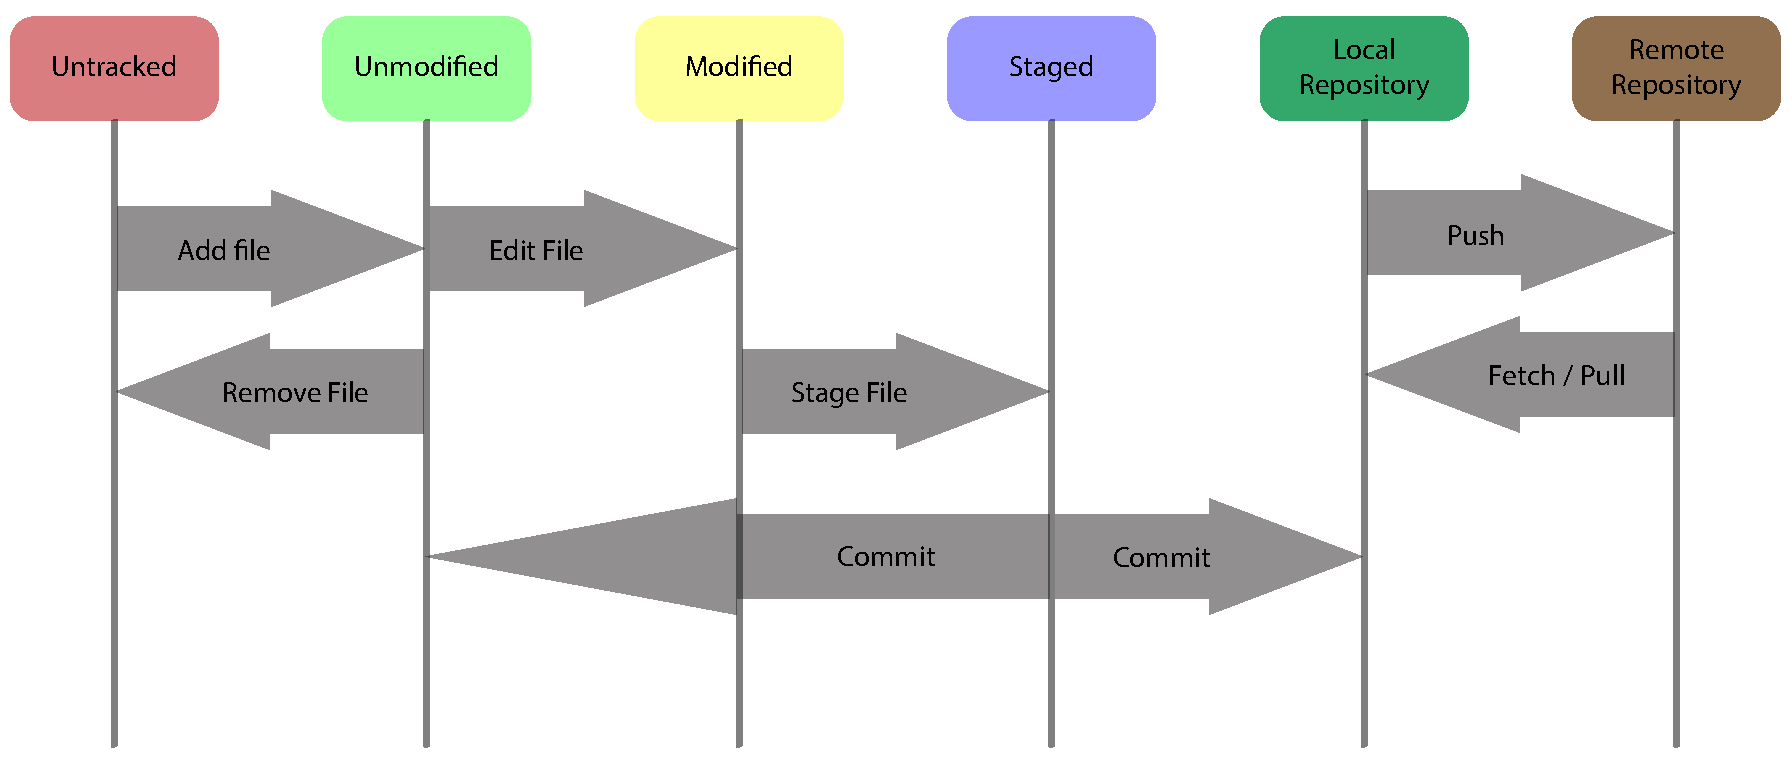
\includegraphics[width=\textwidth]{github.pdf}
\end{figure}



\newpage
\section{The Basics}

\subsection{Adding files}
\subsubsection{For the first time}
When you have created a Git repo, you add new files to it by running
\begin{verbatim}
git add [filename]
\end{verbatim}
or, if you wish to add all files in your current directory and sub-directories, run
\begin{verbatim}
git add *
\end{verbatim}
These files will now be tracked by GitHub, and considered part of your GitHub Repository. Remember that files can exist in your GitHub folder without being added to your repository. Often you wish to keep some files local only.

Deleting a file should remove it both locally and in your GitHub repo.

\subsubsection{Staging files with git add}
When you have done changes to your files, they will need to be \texttt{staged}. This tells GitHub that your changes to this file should be part of your next commit. You stage files by simply running \texttt{git add} on them again. Often you wish to stage all your changes. In that case, you don't have to add them manually. Simply add the "\texttt{a}" flag to your commit(see commits below), and GitHub will stage all changed files for you. (GitHub will of course not stage files that are not in your GitHub repo - aka files you have never run \texttt{git add} on. Such files are always ignored until you \texttt{git add} them).


\subsection{Commits}
A commit represents an official change in your GitHub repository, with an appropriate comment. Others will be able to scroll back through your commits, and see the changes done in each. You can also rewind your work back to an earlier commit, if something went wrong.

\textbf{Commits are probably the most important part of Git to get right.} Here are a few notes.\\
Commits should be done when a new functionality is implemented, a bug is fixed, or some minor changes have been made. Always include a comment in each commit, very briefly explaining what you've done. Avoid doing several larger changes within the same commit (if you are gonna work on something else, do a commit), but also avoid using commit as a save button for each small change you make. If you are continously working on the same thing, no need to commit half-way, unless you're going home for the day, or have reached a natural checkpoint. Commits should also never include code that doesn't work, unless you are on a branch that develops a new feature.

You can do a \textbf{stage} and \textbf{commit} at the same time the following way.
\begin{verbatim}
git commit -am "Example comment. Implemented warp drive function and fixed a unit conversion bug."
\end{verbatim}
The "\texttt{a}" flag tells GitHub to stage all changed files before commiting, and the "\texttt{m}" flag tells that you have included a commit message. If you have done changes you don't wish to commit, you drop the "\texttt{a}" flag, and stage your files manually using \texttt{git add}.

A useful command for getting a view of what files are staged/ustaged and added/not added is
\begin{verbatim}
git status
\end{verbatim}

\subsection{Pushing and pulling- Communicating with remote}
A \textbf{remote repository} is the online repository is stored on GitHubs servers. This is the repository you see by going to GitHubs website. It is associated with an unique URL. Every local repository can also have a unique name for each remote repository it is in contact with. The most important remote repository is, of course, the one mirroring the local repository. This is by default called \texttt{origin}.

When you have done one or more commits, you can push them to your remote repository, such that they are stored on GitHubs servers. The official way of pushing all commited changes is
\begin{verbatim}
git push [remote_repository] [branch_name]
\end{verbatim}
but as long as you are pushing to your \texttt{origin} repository, and you are on master branch, you can simpy run
\begin{verbatim}
git push
\end{verbatim}
which defaults to \texttt{git push origin master}.

When you want to sync your local repository up with your remote one, to get changes done by others or by yourself on other computers, you run a pull command
\begin{verbatim}
git pull [remote_repository] [branch_name]
\end{verbatim}
which again, can be simplified to 
\begin{verbatim}
git pull
\end{verbatim}
under the same circumstances.





\newpage
\section{Forks}
\label{sec:forks}
A fork is a private mirror of someone else's repository. The fork will be an independent repository owned by you, which you can modify freely. Forks are often used to suggest changes to sommeone else's repository, by rewriting some code and submitting a \texttt{Pull Request}, which asks the original owner if they wish to use the changes you made.

\subsection{Setting up a fork}
Press the fork button on the webpage of the GitHub repository you wish to fork. A new repository, owned by you, is now created. Clone the newly created repository as usual.

\subsection{Keeping a fork up to date}
\subsubsection{Setup}
If the original owner makes changes to his repository while you have a fork of it, you usually want these changes. To keep your fork up to date with the original, you must add it as an upstream repository. If you run
\begin{verbatim}
git remote -v
\end{verbatim}
you should see your own github adress as origin fetch and push. To add the upstream repository, run
\begin{verbatim}
git remote add upstream [github_address_of_original_repository]
\end{verbatim}

If you now run \texttt{git remote -v} again, you should see the original repository added as upstream fetch and push.

\subsubsection{Fetching from upstream}
To update your fork with changes done to the master branch upstream, run
\begin{verbatim}
git fetch upstream
\end{verbatim}
Checkout back to your forks master:
\begin{verbatim}
git checkout master
\end{verbatim}
Merge the upstream master with your own master:
\begin{verbatim}
git merge upstream/master
\end{verbatim}


\subsection{Pull Requests}
A Pull Request should be initialized when you want to present your changes to the owner of the original repository. You do this on GitHubs website. The owner can accept your Pull Request, or comment on changes that should be done.


\newpage
\section{Branches}
Your default branch is called \texttt{master}, and should contain the latest of your working code. If you wish to implement a new feature or do larger changes, it's often smart to branch off from master, creating a copy you can work on, which doesn't affect the master code until you merge them. This way, your master branch never has half-done code.

\subsection{Creating a new branch}
To create a new branch, make sure your fork's master is up to date, and run
\begin{verbatim}
git checkout -b [name_of_branch]
\end{verbatim}
This will place you in the new branch.

\subsection{Switching between branches}
Switching between branches in done with
\begin{verbatim}
git checkout [name_of_branch]
\end{verbatim}
Note that this will instantly change all your local files to match the branch you are checking out. This allows you to work on multiple branches at the same time. You can also do changes to master (changes to master won't affect other branches. If you do changes to master, it's often a good idea to merge these changes into your branches. More on this below).

You can see all branches on your fork by running
\begin{verbatim}
git branch
\end{verbatim}

\subsection{Working on the branch}
You \textbf{commit} changes the usual way when on a branch.

If you wish to \textbf{push} your changes to github while on a branch different from master, you must remember to specify the remote repository, and your working branch:
\begin{verbatim}
git push origin [name_of_branch]
\end{verbatim}


\subsection{Fetching master or other branch}
When working on multiple branches in parallel, you often wish to fetch your code-changes from another branch. When on a branch, you can pull changes done on another branch the following way
\begin{verbatim}
git merge [branch_you_wish_to_fetch]
\end{verbatim}

\subsection{Pull requests}
When you have finished implementing everything you were doing in your branch, you should open a Pull Request to merge it with master. If you are the only one working on the repo, you can simply immediately confirm the request. This is both done at the GitHub website.

Make sure to pull after you make the merge, since you do the merge on the website and not locally. You should also delete the branch unless you wish to work further on the speicific functions of that branch. Each branch should only be used for one purpose - do not recycle branches.


\newpage
\section{Useful commands}
Moving files / renaming files, removing files
\begin{verbatim}
git mv [old_file_name_and_location] [new_file_name_and_location]
git rm [file_to_be_deleted]
\end{verbatim}

\section{I fucked up}
\subsubsection{Added a file to repository that should only exist locally}
Removing a file from GitHub repository without removing it locally:
\begin{verbatim}
git rm --cached [file_to_be_removed]
\end{verbatim}


\subsubsection{Commited too early}
When you have already commited, but want to include additional changes to the commit, you do those changes, stage them, and run
\begin{verbatim}
git commit --amend
\end{verbatim}
which will include those changes in the previous commit.


\subsubsection{Unstaging a file}
\begin{verbatim}
git reset HEAD [file_to_be_unstaged]
\end{verbatim}
The file will remain in the repository as a modified unstaged file.


\subsubsection{Undoing changes to a file}
You can revert the changes done to a file since last commit using
\begin{verbatim}
git checkout -- [file_to_be_reset]
\end{verbatim}




\end{document}
\grid
